\chapter{The Secret Cave}

The sun had nearly reached the meridian, and his scorching rays fell
full on the rocks, which seemed themselves sensible of the heat.
Thousands of grasshoppers, hidden in the bushes, chirped with a
monotonous and dull note; the leaves of the myrtle and olive trees
waved and rustled in the wind. At every step that Edmond took he
disturbed the lizards glittering with the hues of the emerald; afar off
he saw the wild goats bounding from crag to crag. In a word, the island
was inhabited, yet Edmond felt himself alone, guided by the hand of
God.

He felt an indescribable sensation somewhat akin to dread—that dread of
the daylight which even in the desert makes us fear we are watched and
observed. This feeling was so strong that at the moment when Edmond was
about to begin his labor, he stopped, laid down his pickaxe, seized his
gun, mounted to the summit of the highest rock, and from thence gazed
round in every direction.

But it was not upon Corsica, the very houses of which he could
distinguish; or on Sardinia; or on the Island of Elba, with its
historical associations; or upon the almost imperceptible line that to
the experienced eye of a sailor alone revealed the coast of Genoa the
proud, and Leghorn the commercial, that he gazed. It was at the
brigantine that had left in the morning, and the tartan that had just
set sail, that Edmond fixed his eyes.

The first was just disappearing in the straits of Bonifacio; the other,
following an opposite direction, was about to round the Island of
Corsica.

This sight reassured him. He then looked at the objects near him. He
saw that he was on the highest point of the island,—a statue on this
vast pedestal of granite, nothing human appearing in sight, while the
blue ocean beat against the base of the island, and covered it with a
fringe of foam. Then he descended with cautious and slow step, for he
dreaded lest an accident similar to that he had so adroitly feigned
should happen in reality.

Dantès, as we have said, had traced the marks along the rocks, and he
had noticed that they led to a small creek, which was hidden like the
bath of some ancient nymph. This creek was sufficiently wide at its
mouth, and deep in the centre, to admit of the entrance of a small
vessel of the lugger class, which would be perfectly concealed from
observation.

Then following the clew that, in the hands of the Abbé Faria, had been
so skilfully used to guide him through the Dædalian labyrinth of
probabilities, he thought that the Cardinal Spada, anxious not to be
watched, had entered the creek, concealed his little barque, followed
the line marked by the notches in the rock, and at the end of it had
buried his treasure. It was this idea that had brought Dantès back to
the circular rock. One thing only perplexed Edmond, and destroyed his
theory. How could this rock, which weighed several tons, have been
lifted to this spot, without the aid of many men?

Suddenly an idea flashed across his mind. Instead of raising it,
thought he, they have lowered it. And he sprang from the rock in order
to inspect the base on which it had formerly stood.

He soon perceived that a slope had been formed, and the rock had slid
along this until it stopped at the spot it now occupied. A large stone
had served as a wedge; flints and pebbles had been inserted around it,
so as to conceal the orifice; this species of masonry had been covered
with earth, and grass and weeds had grown there, moss had clung to the
stones, myrtle-bushes had taken root, and the old rock seemed fixed to
the earth.

\begin{figure}[ht]
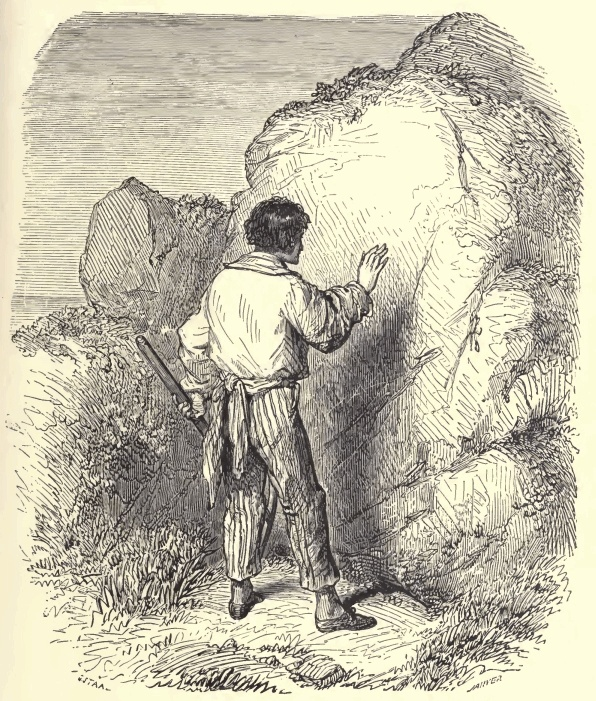
\includegraphics[width=\textwidth]{0301m.jpg}
\end{figure}

Dantès dug away the earth carefully, and detected, or fancied he
detected, the ingenious artifice. He attacked this wall, cemented by
the hand of time, with his pickaxe. After ten minutes’ labor the wall
gave way, and a hole large enough to insert the arm was opened.

Dantès went and cut the strongest olive-tree he could find, stripped
off its branches, inserted it in the hole, and used it as a lever. But
the rock was too heavy, and too firmly wedged, to be moved by anyone
man, were he Hercules himself. Dantès saw that he must attack the
wedge. But how?

He cast his eyes around, and saw the horn full of powder which his
friend Jacopo had left him. He smiled; the infernal invention would
serve him for this purpose.

With the aid of his pickaxe, Dantès, after the manner of a labor-saving
pioneer, dug a mine between the upper rock and the one that supported
it, filled it with powder, then made a match by rolling his
handkerchief in saltpetre. He lighted it and retired.

The explosion soon followed; the upper rock was lifted from its base by
the terrific force of the powder; the lower one flew into pieces;
thousands of insects escaped from the aperture Dantès had previously
formed, and a huge snake, like the guardian demon of the treasure,
rolled himself along in darkening coils, and disappeared.

Dantès approached the upper rock, which now, without any support,
leaned towards the sea. The intrepid treasure-seeker walked round it,
and, selecting the spot from whence it appeared most susceptible to
attack, placed his lever in one of the crevices, and strained every
nerve to move the mass.

The rock, already shaken by the explosion, tottered on its base. Dantès
redoubled his efforts; he seemed like one of the ancient Titans, who
uprooted the mountains to hurl against the father of the gods. The rock
yielded, rolled over, bounded from point to point, and finally
disappeared in the ocean.

On the spot it had occupied was a circular space, exposing an iron ring
let into a square flag-stone.

Dantès uttered a cry of joy and surprise; never had a first attempt
been crowned with more perfect success. He would fain have continued,
but his knees trembled, and his heart beat so violently, and his sight
became so dim, that he was forced to pause.

This feeling lasted but for a moment. Edmond inserted his lever in the
ring and exerted all his strength; the flag-stone yielded, and
disclosed steps that descended until they were lost in the obscurity of
a subterraneous grotto.

Anyone else would have rushed on with a cry of joy. Dantès turned pale,
hesitated, and reflected.

“Come,” said he to himself, “be a man. I am accustomed to adversity. I
must not be cast down by the discovery that I have been deceived. What,
then, would be the use of all I have suffered? The heart breaks when,
after having been elated by flattering hopes, it sees all its illusions
destroyed. Faria has dreamed this; the Cardinal Spada buried no
treasure here; perhaps he never came here, or if he did, Cæsar Borgia,
the intrepid adventurer, the stealthy and indefatigable plunderer, has
followed him, discovered his traces, pursued them as I have done,
raised the stone, and descending before me, has left me nothing.”

He remained motionless and pensive, his eyes fixed on the gloomy
aperture that was open at his feet.

“Now that I expect nothing, now that I no longer entertain the
slightest hopes, the end of this adventure becomes simply a matter of
curiosity.” And he remained again motionless and thoughtful.

“Yes, yes; this is an adventure worthy a place in the varied career of
that royal bandit. This fabulous event formed but a link in a long
chain of marvels. Yes, Borgia has been here, a torch in one hand, a
sword in the other, and within twenty paces, at the foot of this rock,
perhaps two guards kept watch on land and sea, while their master
descended, as I am about to descend, dispelling the darkness before his
awe-inspiring progress.”

\begin{figure}[ht]
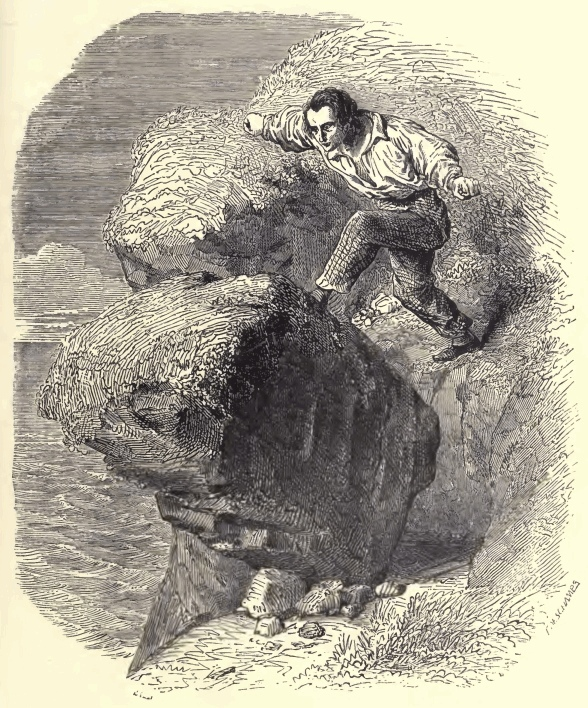
\includegraphics[width=\textwidth]{0303m.jpg}
\end{figure}

“But what was the fate of the guards who thus possessed his secret?”
asked Dantès of himself.

“The fate,” replied he, smiling, “of those who buried Alaric, and were
interred with the corpse.”

“Yet, had he come,” thought Dantès, “he would have found the treasure,
and Borgia, he who compared Italy to an artichoke, which he could
devour leaf by leaf, knew too well the value of time to waste it in
replacing this rock. I will go down.”

Then he descended, a smile on his lips, and murmuring that last word of
human philosophy, “Perhaps!”

But instead of the darkness, and the thick and mephitic atmosphere he
had expected to find, Dantès saw a dim and bluish light, which, as well
as the air, entered, not merely by the aperture he had just formed, but
by the interstices and crevices of the rock which were visible from
without, and through which he could distinguish the blue sky and the
waving branches of the evergreen oaks, and the tendrils of the creepers
that grew from the rocks.

After having stood a few minutes in the cavern, the atmosphere of which
was rather warm than damp, Dantès’ eye, habituated as it was to
darkness, could pierce even to the remotest angles of the cavern, which
was of granite that sparkled like diamonds.

“Alas,” said Edmond, smiling, “these are the treasures the cardinal has
left; and the good abbé, seeing in a dream these glittering walls, has
indulged in fallacious hopes.”

But he called to mind the words of the will, which he knew by heart.
“In the farthest angle of the second opening,” said the cardinal’s
will. He had only found the first grotto; he had now to seek the
second. Dantès continued his search. He reflected that this second
grotto must penetrate deeper into the island; he examined the stones,
and sounded one part of the wall where he fancied the opening existed,
masked for precaution’s sake.

The pickaxe struck for a moment with a dull sound that drew out of
Dantès’ forehead large drops of perspiration. At last it seemed to him
that one part of the wall gave forth a more hollow and deeper echo; he
eagerly advanced, and with the quickness of perception that no one but
a prisoner possesses, saw that there, in all probability, the opening
must be.

However, he, like Cæsar Borgia, knew the value of time; and, in order
to avoid fruitless toil, he sounded all the other walls with his
pickaxe, struck the earth with the butt of his gun, and finding nothing
that appeared suspicious, returned to that part of the wall whence
issued the consoling sound he had before heard.

He again struck it, and with greater force. Then a singular thing
occurred. As he struck the wall, pieces of stucco similar to that used
in the ground work of arabesques broke off, and fell to the ground in
flakes, exposing a large white stone. The aperture of the rock had been
closed with stones, then this stucco had been applied, and painted to
imitate granite. Dantès struck with the sharp end of his pickaxe, which
entered someway between the interstices.

It was there he must dig.

But by some strange play of emotion, in proportion as the proofs that
Faria, had not been deceived became stronger, so did his heart give
way, and a feeling of discouragement stole over him. This last proof,
instead of giving him fresh strength, deprived him of it; the pickaxe
descended, or rather fell; he placed it on the ground, passed his hand
over his brow, and remounted the stairs, alleging to himself, as an
excuse, a desire to be assured that no one was watching him, but in
reality because he felt that he was about to faint.

The island was deserted, and the sun seemed to cover it with its fiery
glance; afar off, a few small fishing boats studded the bosom of the
blue ocean.

Dantès had tasted nothing, but he thought not of hunger at such a
moment; he hastily swallowed a few drops of rum, and again entered the
cavern.

The pickaxe that had seemed so heavy, was now like a feather in his
grasp; he seized it, and attacked the wall. After several blows he
perceived that the stones were not cemented, but had been merely placed
one upon the other, and covered with stucco; he inserted the point of
his pickaxe, and using the handle as a lever, with joy soon saw the
stone turn as if on hinges, and fall at his feet.

He had nothing more to do now, but with the iron tooth of the pickaxe
to draw the stones towards him one by one. The aperture was already
sufficiently large for him to enter, but by waiting, he could still
cling to hope, and retard the certainty of deception. At last, after
renewed hesitation, Dantès entered the second grotto.

The second grotto was lower and more gloomy than the first; the air
that could only enter by the newly formed opening had the mephitic
smell Dantès was surprised not to find in the outer cavern. He waited
in order to allow pure air to displace the foul atmosphere, and then
went on.

At the left of the opening was a dark and deep angle. But to Dantès’
eye there was no darkness. He glanced around this second grotto; it
was, like the first, empty.

The treasure, if it existed, was buried in this corner. The time had at
length arrived; two feet of earth removed, and Dantès’ fate would be
decided.

He advanced towards the angle, and summoning all his resolution,
attacked the ground with the pickaxe. At the fifth or sixth blow the
pickaxe struck against an iron substance. Never did funeral knell,
never did alarm-bell, produce a greater effect on the hearer. Had
Dantès found nothing he could not have become more ghastly pale.

He again struck his pickaxe into the earth, and encountered the same
resistance, but not the same sound.

“It is a casket of wood bound with iron,” thought he.

At this moment a shadow passed rapidly before the opening; Dantès
seized his gun, sprang through the opening, and mounted the stair. A
wild goat had passed before the mouth of the cave, and was feeding at a
little distance. This would have been a favorable occasion to secure
his dinner; but Dantès feared lest the report of his gun should attract
attention.

He thought a moment, cut a branch of a resinous tree, lighted it at the
fire at which the smugglers had prepared their breakfast, and descended
with this torch.

He wished to see everything. He approached the hole he had dug, and
now, with the aid of the torch, saw that his pickaxe had in reality
struck against iron and wood. He planted his torch in the ground and
resumed his labor.

In an instant a space three feet long by two feet broad was cleared,
and Dantès could see an oaken coffer, bound with cut steel; in the
middle of the lid he saw engraved on a silver plate, which was still
untarnished, the arms of the Spada family—viz., a sword, \textit{en pale}, on
an oval shield, like all the Italian armorial bearings, and surmounted
by a cardinal’s hat.

Dantès easily recognized them, Faria had so often drawn them for him.
There was no longer any doubt: the treasure was there—no one would have
been at such pains to conceal an empty casket. In an instant he had
cleared every obstacle away, and he saw successively the lock, placed
between two padlocks, and the two handles at each end, all carved as
things were carved at that epoch, when art rendered the commonest
metals precious.

Dantès seized the handles, and strove to lift the coffer; it was
impossible. He sought to open it; lock and padlock were fastened; these
faithful guardians seemed unwilling to surrender their trust. Dantès
inserted the sharp end of the pickaxe between the coffer and the lid,
and pressing with all his force on the handle, burst open the
fastenings. The hinges yielded in their turn and fell, still holding in
their grasp fragments of the wood, and the chest was open.

\begin{figure}[h]
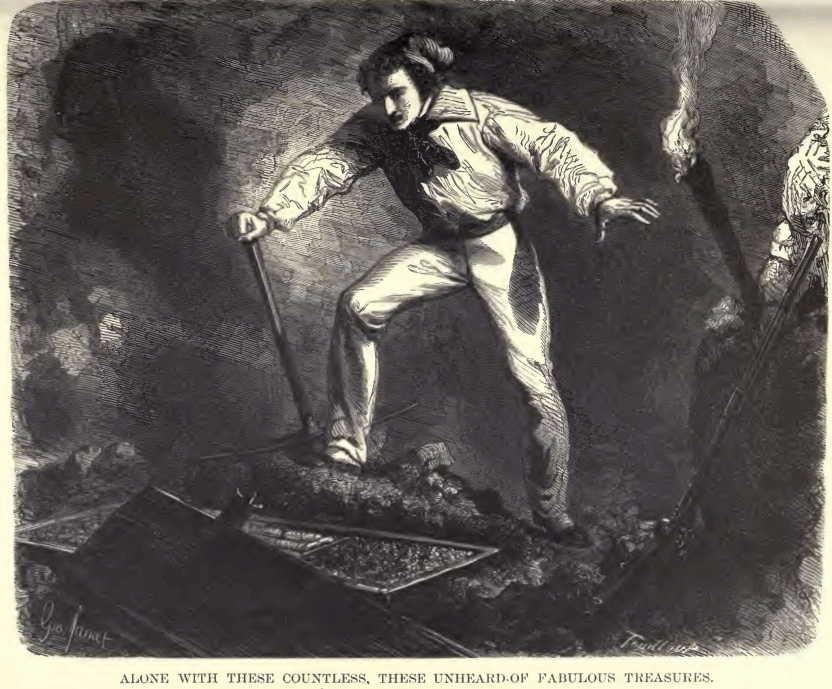
\includegraphics[width=\textwidth]{0307m.jpg}
\end{figure}

Edmond was seized with vertigo; he cocked his gun and laid it beside
him. He then closed his eyes as children do in order that they may see
in the resplendent night of their own imagination more stars than are
visible in the firmament; then he re-opened them, and stood motionless
with amazement.

Three compartments divided the coffer. In the first, blazed piles of
golden coin; in the second, were ranged bars of unpolished gold, which
possessed nothing attractive save their value; in the third, Edmond
grasped handfuls of diamonds, pearls, and rubies, which, as they fell
on one another, sounded like hail against glass.

After having touched, felt, examined these treasures, Edmond rushed
through the caverns like a man seized with frenzy; he leaped on a rock,
from whence he could behold the sea. He was alone—alone with these
countless, these unheard-of treasures! Was he awake, or was it but a
dream? Was it a transient vision, or was he face to face with reality?

He would fain have gazed upon his gold, and yet he had not strength
enough; for an instant he leaned his head in his hands as if to prevent
his senses from leaving him, and then rushed madly about the rocks of
Monte Cristo, terrifying the wild goats and scaring the sea-fowls with
his wild cries and gestures; then he returned, and, still unable to
believe the evidence of his senses, rushed into the grotto, and found
himself before this mine of gold and jewels.

This time he fell on his knees, and, clasping his hands convulsively,
uttered a prayer intelligible to God alone. He soon became calmer and
more happy, for only now did he begin to realize his felicity.

He then set himself to work to count his fortune. There were a thousand
ingots of gold, each weighing from two to three pounds; then he piled
up twenty-five thousand crowns, each worth about eighty francs of our
money, and bearing the effigies of Alexander VI. and his predecessors;
and he saw that the complement was not half empty. And he measured ten
double handfuls of pearls, diamonds, and other gems, many of which,
mounted by the most famous workmen, were valuable beyond their
intrinsic worth.

Dantès saw the light gradually disappear, and fearing to be surprised
in the cavern, left it, his gun in his hand. A piece of biscuit and a
small quantity of rum formed his supper, and he snatched a few hours’
sleep, lying over the mouth of the cave.

It was a night of joy and terror, such as this man of stupendous
emotions had already experienced twice or thrice in his lifetime.
